%-----------------------------------------------------------------------
% Beginning of proc-l-template.tex
%-----------------------------------------------------------------------
%
%     This is a topmatter template file for PROC for use with AMS-LaTeX.
%
%     Templates for various common text, math and figure elements are
%     given following the \end{document} line.
%
%%%%%%%%%%%%%%%%%%%%%%%%%%%%%%%%%%%%%%%%%%%%%%%%%%%%%%%%%%%%%%%%%%%%%%%%

%     Remove any commented or uncommented macros you do not use.

\documentclass{proc-l}

%     If you need symbols beyond the basic set, uncomment this command.
%\usepackage{amssymb}

%     If your article includes graphics, uncomment this command.
%\usepackage{graphicx}

%     If the article includes commutative diagrams, ...
%\usepackage[cmtip,all]{xy}
\usepackage{mathtools} % for \coloneqq
\usepackage{listings} % for \lstlisting
\usepackage[bb=boondox]{mathalfa} % for \mathbb{0}

\usepackage{graphicx}
\graphicspath{ {./images/} }

%     Update the information and uncomment if AMS is not the copyright
%     holder.
%\copyrightinfo{2009}{American Mathematical Society}

\newtheorem{theorem}{Theorem}[section]
\newtheorem{lemma}[theorem]{Lemma}

\theoremstyle{definition}
\newtheorem{definition}[theorem]{Definition}
\newtheorem{example}[theorem]{Example}
\newtheorem{xca}[theorem]{Exercise}

\theoremstyle{remark}
\newtheorem{remark}[theorem]{Remark}

\numberwithin{equation}{section}

\begin{document}

% \title[short text for running head]{full title}
\title[Categorifying the Binomial Theorem]{Categorifying the Binomial Theorem}

%    Only \author and \address are required; other information is
%    optional.  Remove any unused author tags.

%    author one information
% \author[short version for running head]{name for top of paper}
\author{Johnicholas Hines}
\address{}
\curraddr{}
\email{}
\thanks{}

%    author two information
\author{Raymond Cheng}
\address{}
\curraddr{}
\email{}
\thanks{}

%    \subjclass is required.
\subjclass[2020]{Primary }

\date{}

\dedicatory{}

%    "Communicated by" -- provide editor's name; required.
\commby{}

%    Abstract is required.
\begin{abstract}
We try to find a categorification\footnote{https://en.wikipedia.org/wiki/Categorification} of the binomial theorem,
and find some plausible candidates. \({n \choose k}\) might correspond to
\begin{itemize}
    \item sequences of zero or one of length \(n\) containing \(k\) ones, and
    \item functors of ordinals \(\Delta (n-k) \times \Delta k \to \Delta 2\).
    % \item total orders of sets of size \(n\), modulo permutations that fix a subset of size \(k).
\end{itemize} 
\end{abstract}

\maketitle

%    Text of article.
\section{Review of the proof of binomial theorem over Nat}

Let's do a proof of the binomial theorem, and walk through it,
and see how we could do a corresponding categorified version.

We take as `definitional' the Pascal's triangle recursion:
\begin{align*}
{n \choose 0} & \coloneqq 1 \\
{n \choose n} & \coloneqq 1 \\
{n + 1 \choose k + 1} & \coloneqq {n \choose k} + {n \choose k+1}
\end{align*}

We're aiming for this theorem:
\[
(a + b)^n = \sum_{i=0}^n {n \choose i} a^i b^{n-i}
\]

We will prove it inductively.

First we investigate the first few cases of the binomial theorem. In the \(n = 1\) case:
%\begin{align*}
%(a + b)^1 = & a + b \tag{base case of exp} \\ 
%= & 1 \times 1 \times b + 1 \times a \times 1 \tag{1 as identity of product} \\
%= & {1 \choose 0} \times 1 \times b + {1 \choose 1} \times a \times 1 \tag{base case of binomial, twice} \\
%= & {1 \choose 0} \times a^0 \times b^1 + {1 \choose 1} \times a^1 \times b^0 \tag{base cases of exp, four times} \\
%= & {1 \choose 0} \times a^0 \times b^{1-0} + {1 \choose 1} \times a^1 \times b^{1-1} \tag{properties of subtraction?} \\
%= & \sum_{i=0}^n {1 \choose i} * a^i * b^{1-i} \tag{big-sigma introduction?}
%\end{align*}
\begin{align*}
(a + b)^1 = & a + b \\ 
%= & 1  1  b + 1  a  1 \\
%= & {1 \choose 0}  1  b + {1 \choose 1}  a  1  \\
= & {1 \choose 0}  a^0  b^1 + {1 \choose 1}  a^1  b^0  \\
%= & {1 \choose 0}  a^0  b^{1-0} + {1 \choose 1}  a^1  b^{1-1}  \\
= & \sum_{i=0}^n {1 \choose i} * a^i * b^{1-i}
\end{align*}

In the \(n = 2\) case:
%\begin{align*}
%(a + b)^2 & = b^2 + 2 \times a \times b + a^2 \tag{distribution of multiplication over addition} \\
%& = 1 \times 1 \times b^2 + 2 \times a \times b + 1 \times a^2 \times 1 \tag{1 is identity of product} \\
%& = {2 \choose 0} \times a^0 \times b^{2-0} + {2 \choose 1} \times a^1 \times b^{2-1} + {2 \choose 2} \times a^2 \times b^{2-2} \tag{???} \\
%& = \sum_{i=0}^n {2 \choose i} * a^i * b^{1-i} \tag{big-sgima introduction}
%\end{align*}
\begin{align*}
(a + b)^2 & = b^2 + 2  a  b + a^2 \\
% & = 1  1  b^2 + 2  a  b + 1  a^2  1 \\
& = {2 \choose 0}  a^0  b^{2-0} + {2 \choose 1}  a^1  b^{2-1} + {2 \choose 2}  a^2  b^{2-2} \\
& = \sum_{i=0}^n {2 \choose i} * a^i * b^{1-i}
\end{align*}

In the inductive case, we assume that the binomial theorem is true up to a point \(n\), and we show it also is true at \(n+1\). To handwave a bit, we are using the associative, commutative, and distributive properties of addition and multiplication
 to `register' or `align' two sequences of terms, leaving only a couple very simple terms hanging off the two ends.
Once they're aligned we can get the corresponding binomial coefficients to combine using the recursive definition of the binomial coefficients.
Finally we recognize the expression consisting of the simple terms on each side of the simplified middle sequence as an example of the inductive formula we were looking for.
\begin{align*}
(a + b)^{n+1} 
& = (a + b) \times (\sum_{i=0}^n {n \choose i} \times a^i \times b^{n-i}) \\ 
& = (b \times \sum_{i=0}^n {n \choose i} \times a^i \times b^{n-i}) + (a \times \sum_{j=0}^n {n \choose j} \times a^j \times b^{n-j}) \\
& = \left(\sum_{i=0}^n {n \choose i} \times a^i \times b^{n-i+1}\right) + \left(\sum_{j=0}^n {n \choose j} \times a^{j+1} \times b^{n-j}\right) \\
& = b^{n+1} + \sum_{i=1}^n {n \choose i} \times a^i \times b^{n-i+1} + \sum_{i=1}^n {n \choose i+1} \times a^i \times b^{n-i+1} + a^{n+1} \\
& = b^{n+1} + \sum_{i=1}^n \left({n \choose i} \times a^i \times b^{n-i+1} + {n \choose i+1} \times a^i \times b^{n-i+1}\right) + a^{n+1} \\
& = b^{n+1} + \sum_{i=1}^n \left({n \choose i} + {n \choose i+1}) \times a^i \times b^{n+1-i}\right) + a^{n+1} \\
& = {n+1 \choose 0} * a^0 * b^{n-0} + \sum_{i=1}^n ({n+1 \choose i+1} \times a^i \times b^{n+1-i}) + {n+1 \choose n+1} \times a^{n+1} \times b^{n+1-n+1} \\
& = \sum_{i=0}^{n+1} {n+1 \choose i} \times a^i \times b^{n+1-i}
\end{align*}

In doing these algebraic manipulations, I am realizing that I am using the big-sigma indexed sum notation only by imagining expanding the big-sigma indexed sum to a vague large finite binary sum and if it seems plausible according to my imagination (which is grounded in manipulating binary associative-commutative sums)
that a manipulation should be legal, then I take it as legal.

I'm not entirely clear on what axioms license these algebraic manipulations, and big-sigma indexed sum starts to feel like an alien entity, that maybe I should investigate.

\section{What analogies do we have to work with?}

Well, the big three are:
\begin{itemize}
    \item arithmetic product corresponds to cartesian or categorical product,
    \item arithmetic sum corresponds to disjoint union or categorical coproduct, and
    \item arithmetic exponentiation corresponds to the set of functions from one set to another.
\end{itemize}

To categorify the binomial theorem, we want to extend these correspondences with another, ending up with a bijection that `explains'\footnote{In the narrow technical sense that if we take cardinalities of each side of the bijection, we get the
binomial theorem; it's not necessarily a clarifying or helpful explanation.} the binomial theorem, and in particular yields a concrete set of cardinality \({n \choose k}\).

\subsection{The C programming metaphor}

There's a metaphor that I think about, between category theory and and C programming.
(I am assuming some familiarity with programming, programming languages, and C here;
if you are unfamiliar with them, this metaphor will not help.)
In C, there are a few basic types including integers and characters, and a few type constructors, such as arrays,
structs, and unions. Types in programming are a bit like sets in set theory, and a bit like objects in category theory.

Structs in C are a bit like products in set theory, but they're even more similar to mathematical definitions of the form "A \emph{thing} consists of \emph{this}, \emph{that}, and \emph{the other}". The different dimensions do not have a first/second or left/right or 0,1 quality; they have names. Structs are pretty safe and comfortable. 

\begin{lstlisting}[language=C]
struct PointAndLetter {
    int x;
    char c;
};
\end{lstlisting}

Arrays in C are somewhat like  partial functions from Nat to some other type,
which are guaranteed to be defined on some initial section of Nat such as [0..128).
Unlike array types in other languages such as Python or Go the length of the initial section where it is defined
is not normally considered to be accessible from the array itself,
nor is it normally considered feasible to figure out the length of the initial section by
iteratively evaluating larger and larger numbers, since the observable consequence of
attempting to evaluate the array at a point beyond where it is defined is a segmentation fault;
crashing the entire program. So the right thing to do with an array is to communicate the size of the array
via some additional channel. You might define a binary function taking an array and a nat,
that presumes the nat is the length of the array, and sums the contents of the array up to that length.

\begin{lstlisting}[language=C]
int sum(int toSum[], int len) {
    int accum = 0;
    for (int i = 0; i < len; i += 1) {
        accum += toSum[i];
    }
    return accum;
}
\end{lstlisting}

Since the right thing to do is to communicate the size of the array as Nat `beside' the array,
you might describe the type of the array using an `inverse product' notation.
\(\operatorname{Array} X\) is a type somewhat like \((\mathbb{N} \to X) / \mathbb{N}\), or \(X^* / \mathbb{N}\), where we are using Kleene star to mean the type constructor for finite lists. That is, it's a type that, if you took a cross product between this type and \(\mathbb{N}\),
might act a bit like a function \(\mathbb{N} \to X\) (but you have to promise not to evaluate it on values beyond the size) or like \(X^*\), the set of finite lists of \(X\).

Similarly, unions in C are not as safe and convenient as tagged unions in other programming languages,
or coproducts in category theory. They're a bit like untagged unions in set theory.
If you have some types and some names for them, you can construct the union type
(just like if you have some types and some names for them, you can construct the struct type).
If you have an element of any of those types, there is a standard map into the union type
(like a coproduct). However, you cannot in general inspect a union in order to determine which
thing it came from. So right thing to do is to communicate a union together with a `tag' or `kind' field, often in a struct.

\begin{lstlisting}[language=C]

struct TaggedIntOrChar {
    enum {INT, CHAR} kind;
    union {
        int x;
        char c;
    }
};
\end{lstlisting}

Similar to Array, you might describe Union as resulting in some sort of `inverse product',
where you can't do much with a bare union. If you combine it with a kind field,
it acts like a coproduct. `Union of Int and Char' is a type somewhat 
like \((\operatorname{Int} + \operatorname{Char}) / (1 + 1)\).

The point of this meandering about datatypes is to motivate or ground the stuff that we're trying to do later.

We are hoping to:
\begin{enumerate}
\item View a coproduct as a product of a tag and a residual type, with the property that elements of the residual can be `rehydrated' or `decompressed' that is, combined with a corresponding tag, to yield the original element of the coproduct.
\item Build data structures out of tags.
\end{enumerate}

\subsection{The Memory metaphor}
In defining a function, it's sometimes valuable to imagine an array of face-down cards, like the game of Memory. We want to define a procedure where we turn over a few specific cards, and then, 
based on what we see, move the remaining face-down cards around without looking at them.

In writing a proof, `turning over a card' corresponds to analysis by cases. In writing a program, `turning over a card' corresponds to pattern matching or definition by cases. In writing a proof, `moving a card without turning it over` means doing something like applying an existing function, or pre or post composing a function to yield another function. In writing a program, `moving a card without turning it over` corresponds to a variable being introduced and then used without being decomposed by pattern matching. 

\subsection{The Lattice Path metaphor}

There's a standard metaphor or story regarding binomial coefficients, that they count how many ways it is to get to a point on a grid, via, for example, `north' and `east' steps; Pascal's Triangle makes the correspondence very clear. Can we build something relating the lattice path metaphor to something? Visualizing the path as extending from the left corner of a diamond to the right corner, maybe we can `shade in' the left side of the path, and say that a lattice path corresponds to a partition of a product of chains into an upper and a lower set? And a partition of a poset into an upper and lower set corresponds to a monotone map to the chain of length 2? 

(Alternately, maybe we draw the lattice path going `up and down' the diamond, and get a correspondence from binomial coefficients to maximal chains in a poset that is a product of chains?)

Examples:
\begin{itemize}
    \item \({2 \choose 1}\) = 2 = number of maps \(\Delta 1 \times \Delta 1 \to \Delta 2\)
    \item \({3 \choose 1}\) = 3 = number of maps \(\Delta 1 \times \Delta 2 \to \Delta 2\)
    \item \({3 \choose 2}\) = 3 = number of maps \(\Delta 2 \times \Delta 1 \to \Delta 2\)
    \item \({4 \choose 1}\) = 4 = number of maps \(\Delta 3 \times \Delta 1 \to \Delta 2\)
    \item \({4 \choose 2}\) = 6 = number of maps \(\Delta 2 \times \Delta 2 \to \Delta 2\)
    \item \({4 \choose 2} = {3 \choose 1} + {3 \choose 2} = 6\)

    \item Conjecture: \({n \choose k}\) = number of maps from \(\Delta (n - k) \times \Delta k \to \Delta 2\)
\end{itemize}


So it's plausible, since the cardinalities look right, that there might be a natural correspondence. Given a map, say \(3 \times 4 \to 2\), how would you `read it out' in order to define a function from, say, \(A^3 \times B^4 \to (A + B)^7\)? \marginpar{This `read out' function looks to a programmer like a kind of interpreter.}

\section{Lifting the High School Identities}

%TODO: a canonical bijection is an explicitly given map (we're not asking the reader to make a choice) which has an inverse.
%TODO: I am not sure I know how to `work up to unique isomorphism'.

Lifting \(x \times 1 = x\) to Set:

\begin{theorem}
Given a set X, there is a canonical bijection between the categorical product with the singleton set \(X \times 1\) and \(X\).
\end{theorem}

\begin{proof}
The projection to \(X\) has an inverse: \(x \in X \mapsto (x, *)\). 
\end{proof}

Lifting \(x^1 = x\) to Set:

\begin{theorem}
Given a set X, there is a canonical bijection between \(1 \to X\), the set of functions from the singleton set, and X.
\end{theorem}

\begin{proof}
A function from the singleton is a set containing a single pair, the first element of which is \(*\). \({(*, x)} \in 1 \to X \mapsto x\) and \(x \in X \mapsto {(x, *)}\) are the bijection.
\end{proof}

Lifting \(1^x = 1\) to Set:

\begin{theorem}
Given a set \(X\), there is a canonical bijection between \(X \to 1\), the set of functions from \(X\) to the singleton set, and the singleton set.
\end{theorem}

\begin{proof}
The only function \(X \to 1\) is the set of pairs \({ (x, *) | x \in X }\); the bijection takes it to \(*\) and back.
\end{proof}

Lifting \(x^0 = 1\) to Set:

\begin{theorem}
Given a set X, there is a canonical bijection between the set of functions from the empty set to X, and the singleton set.
\end{theorem}

\begin{proof}
Functions are sets of pairs, one for each element of the domain. There are zero elements in the domain, if the domain is the empty set. So regardless of what \(X\) is, there is exactly one function from the empty set to \(X\): the empty set, regarded as a set of pairs.
\end{proof}

Lifting \(x \times (y + z) = x \times y + x \times z\) to Set:

\begin{theorem}
Given sets X, Y, Z, there is a canonical bijection between \(X \times (Y + Z)\) and \(X \times Y + X \times Z\).
\end{theorem}

\begin{proof}
A generic element of \(X \times (Y + Z)\) is a pair, the second part of which has a tag, which we might call either `Y' or `Z'. If it had tag `Y', we map it to `XY'. If it came from `Z', we map it to `XZ'. In the opposite direction, if we get a pair that was tagged with `XY', we dissect it into its X and Y components, tag the Y component with `Y', and compose to form an element of \(X \times (Y + Z\), and treat a pair that was tagged with `XZ' similarly. 
\end{proof}

There are more of these `lifted high school identities', but I worry that the details of how I prove them matter, for building on top of them.

\section{Regarding how to use Fancy Coproducts}

Let's talk about what we need to do with Fancy Coproducts.

The last move that we did in the arithmetic proof was
to go from a coproduct of some things and a Fancy Coproduct over one set of indexes, to a fancy coproduct over a bigger set of indexes.

\[
Coproduct~a + FancyCoproduct~I X = FancyCoproduct~(I+1)~Y
\]

We also did this in reverse, where we took some term out from under the Fancy Coproduct, and reduced the set of indexes to compensate.

Another move that we did in the arithmetic proof was
to go from a coproduct of fancy coproducts with compatible indexes to a fancy coproduct of coproducts.

\[
FancyCoproduct~I X + FancyCoproduct~I Y = FancyCoproduct~I (X + Y)
\]

% Another move that we did (or did we?) was apply a morphism
% of indexes.

Finally, at the base case, we introduced a Fancy Coproduct directly from a Coproduct. I can imagine splitting this into multiple steps,
where first we build a Fancy Coproduct that corresponds to nothing (an initial object is the identity with respect to coproduct?), and then use one of the other moves.





\begin{align*}
(a + b)^1 & = a + b \\ % base case of exponentiation
& = 1 \times 1 \times b + 1 \times a \times 1 \\ % 1 as identity of product
& = {1 \choose 0} a^0 \times b^{1-0} + {1 \choose 1} \times a^1 \times b^{1-1} \\ % base cases of binomial and exponentiation several times
& = \sum_{i=0}^n {1 \choose i} * a^i * b^{1-i} % rule of introduction of summation notation?
\end{align*}


% 4. x * y = y * x
% 5. x * (y + z) = x * y + x * z
% x^1 = x
% 10. (x * y)^z = x^z * y^z
% 11. (x^y)^z = x^{y * z}.

Lifting \((x + y) + z = x + (y + z)\) to Set:

\begin{theorem}
Given sets \(X, Y, Z\), there is a canonical bijection between the categorical coproduct \((X + Y) + Z\) and the categorical coproduct \(X + (Y + Z)\).
\end{theorem}

\begin{proof}
TODO
\end{proof} 


Lifting \(x + y = y + x\) to Set:

\begin{theorem}
Given sets \(X, Y\), there is a canonical bijection between the categorical coproduct \(X + Y\) and the categorical coproduct \(Y + X\).
\end{theorem}

\begin{proof}
TODO
\end{proof}

\section{The substantial section}

\begin{theorem}
Maps \(\Delta i \times \Delta j \to \Delta 2, i > 0, j > 0\) can be put in bijection with \(((\Delta i-1) \times \Delta j \to \Delta 2) + (\Delta i \times \Delta (j-1) \to \Delta 2)\).
\end{theorem}

This corresponds to the recursive part of the definition of binomial numbers.

\begin{proof}
Consider where the functor takes the pair (bottom, top). If (bottom, top) goes to bottom, then the functor also takes (bottom, x) to bottom for all x. If (bottom, top) goes to top, then the functor also takes (x, top) to top.

So the restriction of the domain of the functor doesn't lose any additional information.\marginpar{Note this `doesn't lose information' concept is interesting, and this step is weak!}

So functors \(\Delta i \times \Delta j \to \Delta 2\), where \(i\) and \(j\) are both greater than 0, have a bijection with \(((\Delta i-1) \times \Delta j \to \Delta 2) + (\Delta i \times \Delta (j-1) \to \Delta 2)\). 
\end{proof}

Similarly, strings of zeroes and ones of length \(n\) with \(k\) ones, if \(n > 0\), you can inspect the first (or last) element of the string, and obtain an even more direct correspondence. \(\operatorname{Binstring} (n+1) k = (\operatorname{Binstring} n k) + (\operatorname{Binstring} n (k-1))\)


\begin{theorem}
There is a canonical bijection between \(\Delta i \times \Delta j \to \Delta 2\), that is, monotone maps from a product of a chain of length i and a chain of length j to a chain of length 2, and functions \((\Delta i \to A) \times (\Delta j \to B) \to \Delta (i + j) \to (A + B)\),
that is, functions from pairs of functions from chains of length i to \(A\) and functions from chains of length j to \(B\) to functions from chains of length i + j to the coproduct of \(A + B\).
\end{theorem}

\begin{proof}
We will show this by induction on i and j.

Given a map \(f\),

\begin{itemize}
\item (The first base case) If \(i = 0\), then project the pair to the second component, then compose it with the injection \(B \hookrightarrow (A + B)\).

\item (The second base case) If \(j = 0\), then project the pair to the first component, then compose it with the injection \(A \hookrightarrow (A + B)\).
\end{itemize}

Remaining is the recursive case. Remember in this case we have that \(i, j\) are both greater than zero, and we have the inductive bijection for smaller pairs.
\marginpar{TODO: what do we need regarding the concept of `smaller pairs'?}

We strictly follow the arithmetic proof, wielding the lemmas regarding lifted analogs of the high school identities and fancy coproducts at every step where they were used in the arithmetic
proof.

TODO?

%TODO: what even is this?

%\begin{align*}
%(I \to A) \times (J \to B) \to N \to (A + B) \\
%= \tag{by factoring an A out of \(I \to A\)? Need a lemma for that?} \\
%A \times (I-1 \to A) \times (J \to B) \to N \to (A + B) \\
%= \\
%= \tag{by invoking the canonical bijection recursively} \\
%= \tag{by injecting \(A \to (A + B)\)}
%\end{align*}

%If f takes (I, J) to 1, then
%we use:

%\begin{align*}
%(I \to A) \times (J \to B) \to N \to (A + B) \\
%= \tag{by factoring an A out of \(I \to A\)? Need a lemma for that?} \\
%A \times (I-1 \to A) \times B \times ((J-1) \to B) \to N \to (A + B) \\
%= \tag{by invoking the canonical bijection recursively} \\
%= \tag{by injecting \(A \to (A + B)\)} \\
%\end{align*}

\end{proof}

Since we are using the arithmetic proof so rigidly as a guide for the lifted proof, anything that fits the the base cases and recursive cases of the definition of binomial coefficients, such as \(\operatorname{Binstring}\) would also work.

\section{Extensions}

There is a natural question - if binomials correspond to maps out of pairs, do trinomials correspond to maps out of triples? And I think yes, that is the case. The lattice path becomes a lattice surface spanning six corners of a cuboid, and/or a hexagon tiled with rhombuses. There are two normal ways to decompose a linear string of zeroes and ones, by plucking a boolean off one end or the other. The corresponding decomposition of the hexagon-tiled-with-rhombuses lattice surface has six `ends', the six sides of the cuboid, and you can `pluck' lattice paths off of any of them.

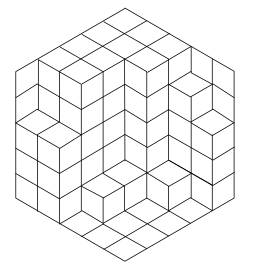
\includegraphics{hexagon}

%    Bibliographies can be prepared with BibTeX using amsplain,
%    amsalpha, or (for "historical" overviews) natbib style.
\bibliographystyle{amsplain}
%    Insert the bibliography data here.

\end{document}

%%%%%%%%%%%%%%%%%%%%%%%%%%%%%%%%%%%%%%%%%%%%%%%%%%%%%%%%%%%%%%%%%%%%%%%%

%    Templates for common elements of a journal article; for additional
%    information, see the file Author_Handbook_Journals.pdf, included
%    in the PROC author package, and the amsthm user's guide, linked
%    from http://www.ams.org/tex/amslatex.html .

%    Section headings
\section{}
\subsection{}

%    Ordinary theorem and proof
\begin{theorem}[Optional addition to theorem head]
% text of theorem
\end{theorem}

\begin{proof}[Optional replacement proof heading]
% text of proof
\end{proof}

%    Figure insertion; default placement is top; if the figure occupies
%    more than 75% of a page, the [p] option should be specified.
\begin{figure}
\includegraphics{filename}
\caption{text of caption}
\label{}
\end{figure}

%    Mathematical displays; for additional information, see the amsmath
%    user's guide, linked from http://www.ams.org/tex/amslatex.html .

% Numbered equation
\begin{equation}
\end{equation}

% Unnumbered equation
\begin{equation*}
\end{equation*}

% Aligned equations
\begin{align}
  &  \\
  &
\end{align}

%-----------------------------------------------------------------------
% End of proc-l-template.tex
%-----------------------------------------------------------------------